\documentclass[conference]{IEEEtran}
\IEEEoverridecommandlockouts
\usepackage{cite}
\usepackage{amsmath,amssymb,amsfonts}
\usepackage{algorithmic}
\usepackage{graphicx}
\usepackage{textcomp}
\usepackage{xcolor}
\usepackage{url}
\def\BibTeX{{\rm B\kern-.05em{\sc i\kern-.025em b}\kern-.08em
    T\kern-.1667em\lower.7ex\hbox{E}\kern-.125emX}}
\begin{document}

\title{MQJL --- Memory-Efficient Long-Context LLM Inference via QJL and Adaptive Layer-Wise Compression}

\author{\IEEEauthorblockN{Bhargav Chirumamilla}
\IEEEauthorblockA{\textit{Johns Hopkins University}}
\and
\IEEEauthorblockN{Xinkai Shen}
\IEEEauthorblockA{\textit{Johns Hopkins University}}
}

\maketitle

\begin{abstract}
Autoregressive large language models (LLMs) materialize growing key--value (KV) activations throughout decoding; for long prompts and multi-turn workloads, KV cache storage and bandwidth—not raw arithmetic throughput—often cap batch size and tokens-per-second. Quantized Johnson--Lindenstrauss (QJL) addresses long-context KV pressure by preconditioning keys with a random Gaussian sketch, retaining only sign bits of the sketch, and combining the result with unquantized query sketches through an asymmetric inner-product estimator. This design avoids full-precision quantization constants (scale and zero-point metadata) that inflate effective bits per element in classical block-wise KV quantization. At a high level, QJL inherits Johnson--Lindenstrauss intuition: approximation error scales with sketch dimension \(m\) and concentration parameters, yielding unbiased inner-product estimates for attention logits together with probabilistic distortion control.

We summarize QJL formalism and its proved guarantees (Lemma~3.2 unbiasedness and Lemma~3.5 tails in the original formulation~\cite{zandieh2024qjl}), then present \emph{A-QJL}, our adaptive extension: transformer depth is partitioned into \(g{\geq}3\) contiguous layer groups, each using the identical QJL primitive but independent sketch widths \(m_j\), optionally chosen under a fixed surrogate bit budget. Allocation can be hand-tuned (strong baseline) or driven by lightweight calibration signals such as per-layer key-projection variance, with a roadmap toward effective-rank, attention-map, and gradient-based proxies. We document an open-source fork built on the reference QJL CUDA stack, LongBench-style evaluation scripts, and aggregate metrics export for plotting. We emphasize scope: per-group QJL theory applies within each group; end-to-end guarantees for heterogeneous widths across all layers remain open. Empirical tables in this draft are placeholders pending complete GPU sweeps.
\end{abstract}

\begin{IEEEkeywords}
Large language models, KV cache quantization, Johnson--Lindenstrauss transform, randomized sketching, asymmetric estimation, adaptive layer-wise compression, long-context inference, attention mechanism
\end{IEEEkeywords}

\section{Introduction}
\label{sec:intro}
\noindent
Transformer decoders generate text autoregressively: at step $t$, each attention layer forms a query vector $q_\ell^{(t)}$ and computes attention over all previously seen keys $\{k_\ell^{(i)}\}_{i\le t}$ and values $\{v_\ell^{(i)}\}_{i\le t}$ stored in a key--value (KV) cache. This cache avoids recomputing past activations and is therefore central to high-throughput decoding. However, KV storage grows linearly with the context length $n$ and the number of layers $L$, creating a dominant memory footprint and a bandwidth bottleneck for long-context inference~\cite{zandieh2024qjl}. Concretely, for decoder-only LLMs the per-token KV footprint scales with $L$, the number of (KV) heads, and the head dimension, and must be streamed repeatedly from device memory during decoding. As a back-of-the-envelope illustration, a 7B-class model with roughly $L{=}32$ layers, $32$ heads, head dimension $128$, storing both keys and values in FP16, requires on the order of hundreds of kilobytes of KV state per generated token; at $32$K tokens this can reach many gigabytes of cache for a single sequence. As context windows grow from a few thousand tokens toward tens of thousands, this cost becomes a first-order constraint on batch size, latency, and even feasibility on commodity GPUs.

\noindent
A standard approach is to quantize KV tensors to fewer bits. Yet classical block quantization for activations typically stores per-block scales and (optionally) zero-points in higher precision, which can add non-negligible metadata overhead per quantized value depending on block size. In the KV-cache setting, where the stored tensors are large and accessed frequently, even ``only'' one to two extra bits per number can significantly reduce the effective compression ratio and add compute for dequantization~\cite{zandieh2024qjl}. This motivates randomized sketching methods that compress keys in a data-oblivious way without per-block constants.

\noindent
Quantized Johnson--Lindenstrauss (QJL)~\cite{zandieh2024qjl} provides such a route by combining a JL-style random projection with extreme (1-bit) sign quantization of the projected \emph{keys}. The key technical idea is an \emph{asymmetric} estimator for query--key inner products: queries are projected but not sign-quantized, while keys are stored as sign bits of their sketches, enabling an unbiased estimator of $\\langle q,k\\rangle$ with JL-like concentration guarantees. This estimator is tailored to attention where logits depend on dot products and errors can be amplified by the softmax. The paper further demonstrates an efficient CUDA implementation and practical handling of outlier channels in deeper layers.

\noindent
From a randomized-algorithms perspective, QJL is appealing because its memory/accuracy trade-off is governed by sketch dimension rather than the ambient embedding dimension: the required sketch width scales like $m=\\tilde{O}(\\varepsilon^{-2}\\log(1/\\delta))$ for inner products and can be budgeted per token so that the total bit-cost depends only logarithmically on the context length~\cite{zandieh2024qjl}. This provides a clean bridge between JL-style concentration and a practical systems bottleneck (KV residency) in modern LLM serving.

\noindent
While QJL establishes a strong baseline, a uniform sketch width across depth is not obviously optimal. Transformer layers are not identical: activation statistics evolve with depth, deeper layers can exhibit outliers, and approximation error may propagate differently depending on where it is introduced~\cite{zandieh2024qjl}. The released QJL implementation already supports a coarse two-tier policy (``initial'' vs.\ ``later'' layers). Our project extends this idea to \textbf{A-QJL}, which partitions layers into $g\\ge 3$ contiguous depth groups and assigns an independent sketch width to each group under a fixed overall memory budget. Intuitively, A-QJL reallocates bits toward layers that are more sensitive to sketching error and reduces bits where additional precision yields diminishing returns. We consider both hand-tuned schedules and lightweight calibration-based allocation using sensitivity proxies (e.g., key-projection variance), with the goal of improving the quality--memory trade-off without changing model weights.

\textbf{Contributions.}
The contributions of this work are:
\begin{itemize}
\item A clear \textbf{algorithmic formulation} of multi-group QJL (A-QJL): layer-index routing to group sketches, sketch-parameter memory accounting, and compatibility with fused CUDA kernels upstream.
\item A \textbf{sensitivity-guided allocation roadmap}: implemented variance proxy atop key projections~\cite{zandieh2024aqjl-repo}; positioning of stronger signals (effective rank~\cite{rudelson2014}, attention-map perturbation~\cite{vitspec2021}, gradient magnitudes~\cite{fpguide2018}) tied to JL theory and mixed-precision folklore.
\item An \textbf{open evaluation harness} (LongBench-style generation, JSON metrics export, aggregate CSV and plotting) suitable for course-scale reproduction on single-GPU environments.
\item \textbf{Honest scope}: we inherit per-group QJL guarantees from~\cite{zandieh2024qjl} but do not claim new uniform bounds on end-to-end network maps under heterogeneous $\{m_j\}$; we flag this as future theory.
\end{itemize}

\noindent
Section~\ref{sec:related} situates KV compression, JL sketching, and adaptive policies. Section~\ref{sec:method} formalizes attention, QJL, and A-QJL. Section~\ref{sec:discussion} discusses implications and failure modes. Section~\ref{sec:novel} lists extensions. Section~\ref{sec:results} specifies experiments. Section~\ref{sec:conclusion} concludes.

\section{Related Work}
\label{sec:related}

\subsection{KV cache reduction without QJL}

Long-context decoding has stimulated a diverse ecosystem of techniques that shrink or avoid storing full-precision KV tensors. The dominant tension is between \emph{materializing} past activations for fast random access during decode and \emph{recomputing} them to save memory---IO-aware attention kernels tilt this trade-off toward fewer HBM round-trips at the cost of more arithmetic when the sequence fits in SRAM-style tiling, but materialized KV remains the default for long histories where recomputation would dominate~\cite{zandieh2024qjl,touvron2023llama}.

Architectural approaches reduce KV head replication at the expense of representational redundancy (multi-query and grouped-query attention)~\cite{shazeer2019mqa}; they shrink the per-layer KV footprint multiplicatively but do not change the linear-in-\(n\) scaling with context length. Scheduling approaches evict or compress ``less important'' past tokens according to heuristic importance scores or budgeted retention policies---useful when not all indices contribute equally---but can interact badly with causality-sensitive tasks and often require careful calibration to avoid catastrophic forgetting of salient early evidence~\cite{bai2023longbench}. Systems stacks offload KV to CPU memory, NVMe, or tiered paging; these methods lower resident GPU DRAM but incur latency penalties, bandwidth caps on PCIe/NVLink, and synchronization complexity that is orthogonal to algebraic approximation of dot products~\cite{presentation_mqjl}.

Closer to numerical compression are low-bit activation caches: recent KV-oriented quantizers emphasize per-token or per-channel scales (asymmetric layouts) and sometimes separate treatment of keys and values~\cite{kivi2024}; complementary work investigates improved channel clustering, outlier isolation, and numerical stability under aggressive codes~\cite{kvquant2023}. Compared with sketching-first methods, quantization-first pipelines routinely store bookkeeping metadata beside packed codes; block size trades resolution against metadata amortization~\cite{kivi2024}. \textbf{A-QJL is complementary}: it targets randomized linear-algebra surrogates for dot products directly and inherits QJL's low-overhead key representation; it does \emph{not} supersede orthogonal improvements such as eviction, MQA/GQA, or offloading---those can be composed for extremely long horizons~\cite{shazeer2019mqa,zandieh2024qjl}.

\subsection{Johnson--Lindenstrauss and streaming sketches}

Johnson--Lindenstrauss~\cite{jl1984} and successors show that Euclidean geometry of finite point collections can survive aggressive dimension reduction with randomized linear maps controlled by logarithmic distortion parameters. The classical view bounds pairwise distance preservation; extensions address subspace embeddings, fast transforms with structured randomness, and stable-rank refinements where effective dimension replaces ambient \(d\) in sample complexity~\cite{woodruff2014,rudelson2014}. Subsequently, sketches became core tools for streaming algorithms (e.g., Count--Sketch for heavy hitters, Frequent Directions for covariance tracking), randomized regression, approximate matrix multiplication, and sublinear probing of large covariance structures~\cite{woodruff2014}.

Typical JL analyses bound \(\ell_2\) distortion, operator norms, or covariance errors; estimating \emph{bilinear forms} \(\langle q,k\rangle\) faithfully under \emph{extreme} subsequent quantization (retaining only signs of projected keys) differs materially from guaranteeing only \(\|\cdot\|_2\) norm preservation or subspace embeddings of a fixed basis~\cite{zandieh2024qjl}. QJL therefore sits at the intersection of random projection theory and communication-style one-bit quantization: the asymmetric ``Alice compresses radically; Bob retains side information'' pattern mirrors the roles of stored keys versus live queries in attention~\cite{zandieh2024qjl}. Concentration tools familiar from Hanson--Wright and decoupling inequalities~\cite{rudelson2014,woodruff2014} inform intuition about variance--dimension trade-offs even when end-to-end network Lipschitz surrogates remain informal~\cite{lipschitz2024}.

\subsection{QJL: algorithm and guarantees}

We briefly recall the centerpiece results of Zandieh et al.~\cite{zandieh2024qjl}: (i)~the quantized map \(H_S(k)=\mathrm{sign}(Sk)\) compactly stores \(\pm 1\) bits of \(Sk\) (plus packing); (ii)~the asymmetric \(\mathrm{Prod}_{\mathrm{QJL}}(q,k)\) recovers \(\langle q,k\rangle\) unbiasedly (\textbf{Lemma~3.2}); (iii)~concentration of deviation around the mean delivers high-probability control \(|\mathrm{Prod}_{\mathrm{QJL}}-\langle q,k\rangle|\leq \varepsilon\|q\|_2\|k\|_2\) when sketch width \(m\) scales polynomially like \(\varepsilon^{-2}\log(1/\delta)\) (\textbf{Lemma~3.5}); (iv)~\textbf{Theorem~3.6} aggregates pairwise controls to relative multiplicative error on softmax pre-logits requiring roughly \(m\approx \varepsilon^{-2}\log n\) bits per retained key token (\(n\) context length), emphasizing \emph{dimension-independent} asymptotics in embedding size \(d\).

Relative to generic JL maps, QJL is engineered for the attention inner-product kernel: unbiased logits stabilize gradient-free decoding under softmax~\cite{zandieh2024qjl}, while sign-only keys minimize stored bandwidth per position. Auxiliary engineering contributions include fused CUDA kernels, stable handling of outliers in deeper transformer layers via split inlier/outlier projections, and strong empirical fidelity on Llama-scale models~\cite{zandieh2024qjl,qjlkernel}. Open-source kernels~\cite{qjlkernel} and follow-on forks that expose multi-group schedules~\cite{zandieh2024aqjl-repo} matter for reproducibility: theory-level lemmas assume idealized Gaussian \(S\); practice adds RNG amortization, packing layouts, and kernel fusion constraints that shape feasible \(\{m_j\}\) lattices~\cite{presentation_mqjl}.

\subsection{Layer-wise and adaptive inference policies}

Layer-wise mixed precision originated for \emph{parameters} and training dynamics~\cite{fpguide2018}; analogous ideas adaptively downgrade activations selectively by signal-to-noise heuristics, gradient sensitivity, or hardware throughput~\cite{fpguide2018}. At inference KV compression time, comparatively fewer principled depth-allocation maps are documented openly: QJL's two-band policy (large projection for earliest layers, narrower later)~\cite{zandieh2024qjl} is a strong default but does not exhaust the space of monotone or non-monotone \(\mathbf{m}\) vectors under a global bit budget~\cite{zandieh2024aqjl-repo}.

Temporal and positional hybrids (sliding-window exact attention over recent tokens fused with chunked or summarized distant history, or extended-context positional recipes)~\cite{longrope2024} orthogonalize fidelity along the \emph{token} axis rather than the \emph{depth} axis~\cite{presentation_mqjl}: one can imagine combining windowed attention with depth-stratified QJL so that near-field tokens see exact dot products while far-field keys remain heavily sketched---we leave systematic study to future work~\cite{longrope2024,zandieh2024qjl}. \textbf{A-QJL aligns with randomized resource allocation motifs}: reallocating sketch entropy across heterogeneous depth strata under a monotone global budget parallels water-filling and proportional fairness heuristics in convex allocation, differing mainly in the surrogate objective (task score, proxy variance, or hand-tuned priors~\cite{presentation_mqjl}). Sensitivity to softmax curvature suggests tying allocation to perturbation analysis of attention maps~\cite{vitspec2021}, still nascent for randomized KV codecs.

\subsection{Benchmarks for long-context quality}

Measuring fidelity after aggressive KV compression demands tasks where errors compound across many attended positions and where distractors or multi-hop evidence stress retrieval over long spans~\cite{bai2023longbench}. LongBench provides bilingual long-form QA, summarization, and multi-task suites with heterogeneous domain lengths and scoring scripts suited to generative evaluation~\cite{bai2023longbench}; we cite it explicitly because our reproducibility harness targets analogous generation-and-score pipelines (task-specific aggregation, F1-style overlap metrics, and JSON/CSV exports for aggregation~\cite{presentation_mqjl}).

Complementary checks include open-ended perplexity on fixed corpora~\cite{touvron2023llama} and layer-wise activation statistics (e.g., outlier prevalence) that explain when quantization-first vs sketch-first methods diverge~\cite{kvquant2023,kivi2024}. Reporting should separate \emph{prefill} vs \emph{decode} regimes when latency-sensitive: some benchmarks stress prompt-heavy prefill, others multi-turn decode~\cite{bai2023longbench,presentation_mqjl}. We emphasize that a single scalar score rarely captures tail failures (e.g., dropped entities in long summaries); error analysis and stratification by sequence length deciles remain best practice~\cite{bai2023longbench}.

\section{Methodology}
\label{sec:method}

\subsection{Problem setting}
\label{sec:problem}

Consider a decoder-only stack with $L$ layers indexed by \(\ell\in\{0,\ldots,L-1\}\) (Llama-style codebases). Inference has two regimes: \emph{(i)~prefill}---process all prompt tokens once to initialize caches; \emph{(ii)~decode}---append one token at a time while reading the full KV history. Throughout, each attention block maps hidden states into queries, keys, and values via learned linear maps; RoPE~\cite{touvron2023llama} or related positional embeddings apply before cache append. Let \(H_{\mathrm{kv}}\) denote the number of key--value heads (GQA/MQA replicate or share keys across query heads to shrink KV bandwidth~\cite{shazeer2019mqa}); \(d\) is the per-head key/query dimension.

For batch size one and a single representative KV head (fused kernels tile over heads and batches~\cite{zandieh2024qjl,qjlkernel}), let \(q_\ell^{(t)}, k_\ell^{(i)}\in\mathbb{R}^d\) be the query at decode step \(t\) and the cached key at token index \(i\) in layer \(\ell\). Causal masking enforces locality: only \(i\le t\) participate~\cite{zandieh2024qjl}.
\begin{equation}
\alpha_{\ell}(t,i) \;=\; \frac{(q_\ell^{(t)})^\top\, k_\ell^{(i)}}{\sqrt{d}} \quad\text{for } i\le t .
\end{equation}
The attention output aggregates values $v_\ell^{(i)}\in\mathbb{R}^{d_v}$ (typically \(d_v{=}d\)) with $p_{\ell}(t,i)\propto \exp \big(\alpha_{\ell}(t,i)/\tau\big)$, \(\tau{>}0\) (default \(\tau{=}1\))~\cite{zandieh2024qjl}. Errors in \(\hat{\alpha}_{\ell}(t,i)\) feed a Lipschitz map in \(\alpha\mapsto \mathrm{softmax}(\alpha)\); logits near the decision boundary of the mass distribution are disproportionately sensitive~\cite{vitspec2021}, which motivates \emph{unbiased} dot-product surrogates and depth-aware control of sketch noise.

\textbf{Residency model.} Materializing FP16 (or BF16) keys and values for all layers scales linearly in context length \(n\), layers \(L\), heads \(H_{\mathrm{kv}}\), and vector width~\cite{touvron2023llama,zandieh2024qjl}. Prefill dominates compute once per prompt; decode repeatedly reads the entire KV history for each new token, so HBM traffic to the cache often dominates latency at long \(n\)~\cite{zandieh2024qjl,presentation_mqjl}. QJL compresses the \emph{key} stream entering the dot product; values may use an orthogonal codec (e.g., per-token low-bit quantization~\cite{kivi2024}). We suppress batch index \(B{>}1\) unless noted; resident cache scales roughly linearly in \(B\)~\cite{presentation_mqjl}.

Exact storage persists full-precision $\{k_\ell^{(i)}, v_\ell^{(i)}\}$ for each cached \(i\) at every \(\ell\)~\cite{zandieh2024qjl}. \textbf{Objective.} Replace or compress keys (optionally values) while controlling task metrics \(\mathcal{M}\), subject to a global KV memory budget \(\mathcal{V}\) (peak \texttt{CUDA} allocator statistics during decode~\cite{presentation_mqjl}). We do \emph{not} fine-tune base weights~\cite{touvron2023llama}; sketch widths, group boundaries, and calibration draws are inference-time knobs only.

\subsection{Baseline QJL (review)}
\label{sec:qjl}

Figure~\ref{fig:qjl-overview} sketches the key-query projection flow and its placement beside per-token value quantization in a representative KV cache~\cite{zandieh2024qjl,kivi2024}. Fix sketch size $m\ll d$ and a random matrix $S\in\mathbb{R}^{m\times d}$ with IID $\mathcal{N}(0,1)$ entries (rows are independent Gaussian vectors~\cite{zandieh2024qjl}). The same realization \(S\) is reused for all token positions within a layer instantiation so that \(\mathrm{Prod}_{\mathrm{QJL}}\) compares \(q\) and \(k\) in a shared random subspace; fresh draws per layer (or per A-QJL group) decorrelate depth-wise errors~\cite{zandieh2024qjl,zandieh2024aqjl-repo}.

Keys are summarized by $H_S(k)=\mathrm{sign}(Sk)\in\{\pm1\}^m$ (packed to \(\lceil m/8\rceil\) bytes per channel block in kernels~\cite{qjlkernel}); live queries use full-precision $Sq\in\mathbb{R}^m$ at score time. The scalar $\|k\|_2$ appears in~\eqref{eq:prodqjl}: implementations cache an FP16/BF16 norm alongside sign bits so the estimator cancels the cosine bias that would appear if both sides were sign-quantized~\cite{zandieh2024qjl}.
The QJL estimator (Definition~3.1 in~\cite{zandieh2024qjl}) is
\begin{equation}
\mathrm{Prod}_{\mathrm{QJL}}(q,k) \ =\ \frac{\sqrt{\pi/2}}{m}\,\|k\|_2 \, \big\langle Sq,\, \mathrm{sign}(Sk) \big\rangle .
\label{eq:prodqjl}
\end{equation}
\textbf{Unbiasedness.} $\mathbb{E}_S[\mathrm{Prod}_{\mathrm{QJL}}]=\langle q,k\rangle$: symmetric 1-bit quantization of \emph{both} \(Sq\) and \(Sk\) would induce a cosine nonlinearity that biases inner-product recovery; retaining \(Sq\) in full precision while compressing only keys restores unbiasedness (\textbf{Lemma~3.2}~\cite{zandieh2024qjl}).

\textbf{Concentration.} For sufficiently large $m$, $|\mathrm{Prod}_{\mathrm{QJL}}-\langle q,k\rangle|\le \varepsilon \|q\|_2\|k\|_2$ w.p.\ $\ge 1-\delta$, with scaling $m\ge c\,\varepsilon^{-2}\log(1/\delta)$ (explicit constants in Lemma~3.5~\cite{zandieh2024qjl}). Intuitively, larger \(m\) reduces variance of the random sign correlation \(\langle Sq,\mathrm{sign}(Sk)\rangle\) around its mean.

\textbf{Attention translation.} Theorem~3.6~\cite{zandieh2024qjl} chains Lemma~3.5 across the \(n\) positions attended at a step to bound \emph{relative} multiplicative error on softmax pre-activations; the \(\log n\) factor arises from a union bound over competing keys. This is the primary bridge from linear-algebraic sketch guarantees to decoder stability.

\textbf{Systems.} The reference stack packs sign bits, optionally splits inlier/outlier channels with a second sketch and separate norms~\cite{zandieh2024qjl}, and exposes fused CUDA kernels for quantize and score phases~\cite{zandieh2024qjl,qjlkernel}. Reference \texttt{QJLSketch} modules store projection directions as \texttt{torch.randn((d,m))} with optional QR rotation and Walsh--Hadamard composition for throughput~\cite{qjlkernel,zandieh2024aqjl-repo}. Typical deployment pairs QJL keys with a separate value-cache quantizer~\cite{kivi2024}.

\begin{figure}[t]
\centering
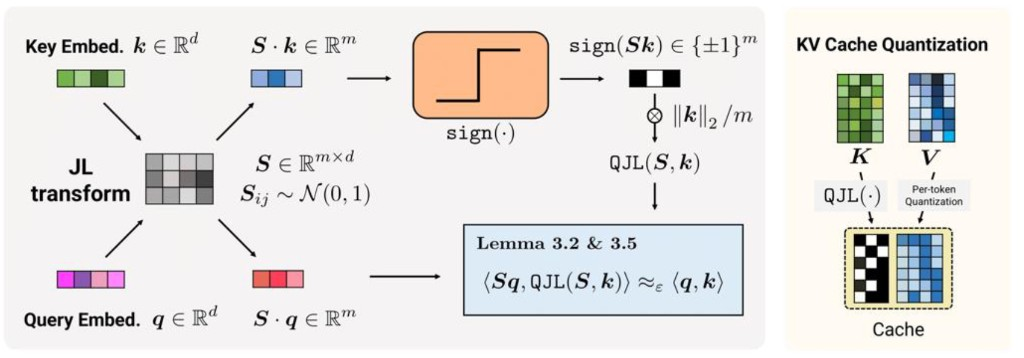
\includegraphics[width=\linewidth]{figures/qjl_kv_overview.png}
\caption{Schematic of QJL in a KV-cache setting~\cite{zandieh2024qjl}. Gaussian $S\in\mathbb{R}^{m\times d}$ projects keys and queries from $\mathbb{R}^d$ to $\mathbb{R}^m$; cached keys retain only $\mathrm{sign}(Sk)$ while live queries use $Sq$ in the asymmetric estimator~\eqref{eq:prodqjl}, yielding unbiased $\mathbb{E}_S[\mathrm{Prod}_{\mathrm{QJL}}]=\langle q,k\rangle$ (Lemma~3.2) and high-probability error bounds (Lemma~3.5)~\cite{zandieh2024qjl}. Values $V$ are often compressed with an independent low-bit path~\cite{kivi2024}. Diagram from project materials~\cite{presentation_mqjl}.}
\label{fig:qjl-overview}
\end{figure}

\textbf{Operational sketch refresh.} Sketches \(\{S^{(j)}\}\) are drawn once per group (or once per layer in the vanilla stack) and held fixed for the lifetime of the session so that cached \(\mathrm{sign}(S^{(j)}k)\) stays consistent with future queries~\cite{zandieh2024qjl,zandieh2024aqjl-repo}. RNG seeds must be logged for reproducibility across machines~\cite{presentation_mqjl}. Optional QR rotation of Gaussian blocks and randomized Walsh--Hadamard chains approximate orthogonal/subgaussian maps discussed in~\cite{zandieh2024qjl} and trade statistical sharpness for arithmetic intensity in the fused CUDA kernels~\cite{qjlkernel}. Changing \(S\) mid-session invalidates the cache unless all keys are re-encoded.

\subsection{QJL guarantees inherited by each A-QJL group}
\label{sec:guarantees}

\textbf{Per-layer, per-sketch.}
Fix group $j$ using dimension $m_j$ and an independently drawn sketch $S^{(j)}$. For any pair $(q,k)$ whose logits are computed with that group's maps, \eqref{eq:prodqjl} with $(S,m)\leftarrow (S^{(j)}, m_j)$ satisfies \textbf{Lemma~3.2} (unbiasedness) and \textbf{Lemma~3.5} (tails) exactly as in~\cite{zandieh2024qjl}, provided the same distributional assumptions on $S^{(j)}$ and the stated $(m_j,\varepsilon,\delta)$ regime hold. Independence of $\{S^{(j)}\}$ means per-group failure events can be union-bounded separately; dependence across \emph{depth} enters only through the network map, not through shared randomness across groups.

\textbf{What we do \emph{not} claim.}
We do \emph{not} assert that a vector $(m_1,\ldots,m_G)$ minimizing a proxy of KV bytes also minimizes cross-entropy on a downstream task, nor a single theorem that heterogeneous widths minimize a global functional of logits or likelihoods. Attention, layer normalization, MLPs, and residuals compose nonlinearly; perturbations on early logits can be amplified or dampened later~\cite{lipschitz2024}. End-to-end Jacobian-style bounds under realistic smoothness assumptions remain future theory.

\textbf{Operational guarantee statement (informal).}
If each $m_j$ meets the Lemma~3.5 scale for a per-pair tolerance $(\varepsilon,\delta')$, then within group $j$ the QJL surrogate is individually well behaved; composing $G$ groups still leaves cross-layer interactions uncharacterized, so we rely on LongBench-style empirical arbitration~\cite{bai2023longbench,presentation_mqjl} in addition to these local lemmas.

\subsection{Multi-group routing (A-QJL)}
\label{sec:aqjl}

Partition depths with strictly increasing breakpoints \(r_1<\cdots<r_{G-1}\) in \(\{1,\ldots,L-1\}\), sentinels \(r_0=0\) and \(r_G=L\), and zero-based layer indices \(\ell\in\{0,\ldots,L-1\}\). Layer \(\ell\) lies in group \(j\in\{0,\ldots,G-1\}\) iff \(r_j\le \ell < r_{j+1}\) (half-open intervals). Thus there are exactly \(G\) contiguous strata; each stratum instantiates an independent sketch \(S^{(j)}\in\mathbb{R}^{m_j\times d}\) and applies~\eqref{eq:prodqjl} with \((S^{(j)},m_j)\) to every attention score in layers \(\ell\) of that stratum~\cite{zandieh2024aqjl-repo}. Outlier masks and dual-sketch branches follow the upstream policy independently per group.

\textbf{Interface mapping.} Command-line and JSON configs pass \texttt{layer\_group\_boundaries} as the sorted list \([r_1,\ldots,r_{G-1}]\); the code infers \(r_0\) and \(r_G{=}L\) from the model~\cite{zandieh2024aqjl-repo}. The companion list \texttt{key\_quantization\_bits\_per\_group} supplies \((m_0,\ldots,m_{G-1})\) (implementation naming reflects historical ``bits'' fields; here each entry is the sketch width \(m_j\))~\cite{zandieh2024aqjl-repo,presentation_mqjl}.

\textbf{Architecture-dependent breakpoints.}
Llama-family stacks differ in $L$ (e.g., 7B: $L{=}32$; 13B: $L{=}40$; 70B: $L{=}80$~\cite{touvron2023llama}). Boundaries must satisfy \(0<r_1<\cdots<r_{G-1}<L\); invalid tuples should be rejected at load time. Percentile-based boundaries (Related Work) remap layer indices to equal \emph{sensitivity} mass rather than equal depth counts~\cite{presentation_mqjl}.

\textbf{Concrete example ($L{=}32,G{=}4$).}
Boundaries \texttt{[8,16,24]} yield groups \(\ell\in[0,7]\), \([8,15]\), \([16,23]\), \([24,31]\)~\cite{zandieh2024aqjl-repo}. A monotone width vector \((512,384,256,192)\) allocates more random dimensions to earlier depth where activations are often more variable in pilot runs~\cite{presentation_mqjl}. Increasing any \(m_j\) tightens Lemma~3.5-type control for that stratum at the expense of \(\mathcal{B}\)~\cite{zandieh2024qjl}.

\textbf{Comparison to vanilla two-band QJL.} The publisher baseline exposes \((m_{\mathrm{init}},m_{\mathrm{rest}},L_0)\): one width for ``initial'' layers \(\ell<L_0\) and another thereafter~\cite{zandieh2024qjl}. Setting \(G{=}2\) with \(r_1=L_0\) recovers that factorization; \(G{>}2\) strictly generalizes the policy class. When comparing to A-QJL, match surrogate \(\mathcal{B}\) (or measured peak KV bytes) so gains reflect \emph{where} bits are spent, not only how many~\cite{presentation_mqjl}.

\subsection{Budget-constrained sketch-width selection}
\label{sec:budget}

Let \(\Delta_j=r_{j+1}-r_j\) denote the number of layers in group \(j\). We use a linear surrogate for total key-sketch ``surface area''
\begin{equation}
\mathcal{B}(\mathbf{m})=\sum_{j=0}^{G-1}\Delta_j \, m_j ,
\label{eq:budget}
\end{equation}
which correlates with packed sign-bit volume before outlier side channels (exact byte accounting includes norms, outlier blocks, and alignment padding~\cite{zandieh2024qjl,qjlkernel}). The target \(B_{\mathrm{tgt}}\) is chosen by (i)~matching a reference two-tier QJL configuration's \(\mathcal{B}\), or (ii)~capping peak KV bytes observed in profiling~\cite{presentation_mqjl}. Because CUDA kernels favor aligned tile widths, candidate \(m_j\) are snapped to multiples of \(64\)~\cite{zandieh2024qjl}; snapping can overshoot \(B_{\mathrm{tgt}}\), so a repair pass (greedy shave from lowest-sensitivity groups) may be needed~\cite{presentation_mqjl}.

\textbf{Sensitivity inputs (tiered roadmap).}

\textit{(a) Key-energy proxy (implemented~\cite{zandieh2024aqjl-repo}).}
\texttt{scripts/sensitivity\_profiler.py} registers forward hooks on each layer's \texttt{k\_proj} output, runs a short calibration forward pass, and records per-layer empirical variance of key activations as a magnitude proxy~\cite{presentation_mqjl}. Group weights \(w_j=\sum_{\ell\in\text{stratum }j}\mathrm{Var}_\ell\) (or robust variants) feed proportional or water-filling maps; the script prints ready-to-paste \texttt{--layer\_group\_boundaries} / \texttt{--key\_quantization\_bits\_per\_group} flags~\cite{zandieh2024aqjl-repo}.

\textit{(b) Stable-rank proxy (planned).}
For windowed stacks of projected keys compute $\mathrm{stable\_rank}=(\sum_i \sigma_i)^2/\sum_i \sigma_i^2$~\cite{rudelson2014}, connecting effective dimension to sufficient sketch complexity~\cite{woodruff2014}.

\textit{(c) Perturbative score probe (planned).}
For a small grid of \(\mathbf{m}\) candidates, measure \(\|\mathrm{softmax}(\alpha)-\mathrm{softmax}(\hat{\alpha})\|_1\) on calibration prompts~\cite{vitspec2021}; costly but logits-aligned.

\textit{(d) Gradient proxy (planned).}
Lightweight backprop on \(\mathcal{D}_c\) yields \(\|\partial \mathcal{L}/\partial K_\ell\|\) as sensitivity weights~\cite{fpguide2018}.

\textbf{Allocation rules.}
\textbf{Proportional:} normalize \(w_j\) to probabilities \(p_j\), set draft widths \(\tilde{m}_j \propto p_j\), then snap and repair \(\mathcal{B}\)~\cite{presentation_mqjl}. \textbf{Water-filling:}
\begin{equation}
m_j \ =\ \max\big(m_{\min},\ \lfloor \mu \cdot \mathrm{AGG}_j(s_\ell) - \eta \rfloor_{\text{snap}}\big), \quad \mu\ \mathrm{s.t.}\ \mathcal{B}(\mathbf{m})\le B_{\mathrm{tgt}} .
\end{equation}
Here \(\mathrm{AGG}_j\) is any monotone aggregate of \(\{s_\ell:\ell\in\text{group }j\}\); \(\mu\) is found by one-dimensional search because \(\mathcal{B}\) is linear in \(\mathbf{m}\) pre-snap~\cite{presentation_mqjl}. \textbf{Discrete knapsack / beam search:} enumerate a pruned lattice \(\mathcal{M}\subset\mathbb{Z}_{+}^G\) near a seed schedule to minimize a distortion upper bound or proxy loss~\cite{presentation_mqjl}.

\textbf{Calibration protocol.} (1)~Choose \(\mathcal{D}_c\) (LongBench subset~\cite{bai2023longbench} or private text~\cite{presentation_mqjl}). (2)~Compute per-layer signals \(s_{\ell}^{(w)}\). (3)~Map layers to groups via fixed or percentile boundaries. (4)~Solve for \(\mathbf{m}\) with \(\mathcal{B}\le B_{\mathrm{tgt}}+\epsilon_{\mathrm{snap}}\) using one of the rules above. (5)~Log \((\mathbf{r},\mathbf{m},B_{\mathrm{tgt}},\mathrm{seed})\) in JSON for experiment drivers. (6)~Freeze weights and sketches for evaluation runs~\cite{presentation_mqjl,zandieh2024aqjl-repo}.

\subsection{Implementation notes}
\label{sec:impl}

\textbf{Model wiring.} The fork extends the Llama-style attention path so each layer selects a \texttt{QJLSketch} bundle indexed by \(j=g(\ell)\)~\cite{zandieh2024aqjl-repo}. Each bundle stores Gaussian directions shaped \((d,m_j)\) (head dimension \(\times\) sketch width), optional outlier width \texttt{dim\_outlier}, and flags for QR rotation / randomized Hadamard composition matching upstream \texttt{QJLSketch}~\cite{qjlkernel,zandieh2024aqjl-repo}. At cache append time the kernel quantizes keys; at decode step the kernel scores fresh \(Sq\) against packed signs and cached norms~\cite{zandieh2024qjl,qjlkernel}.

\textbf{Configuration surface.} Two modes coexist: (\emph{a})~\textbf{Legacy two-profile}---\texttt{key\_quantization\_bits}, \texttt{key\_quantization\_bits\_initial\_layers}, \texttt{initial\_layers\_count}; (\emph{b})~\textbf{A-QJL multi-group}---comma-separated \texttt{--layer\_group\_boundaries} and \texttt{--key\_quantization\_bits\_per\_group} passed through \texttt{run\_longbench.py} into the model config~\cite{zandieh2024aqjl-repo}. JSON experiment cards (e.g., \texttt{config/aqjl\_experiments\_3groups.json}) mirror these fields for batch sweeps~\cite{zandieh2024aqjl-repo,presentation_mqjl}.

\textbf{Automation.} \texttt{scripts/aqjl\_experiments.py} expands JSON run matrices, spawns \texttt{run\_longbench.py} with the correct flags, supports dry-run previews, merges per-task JSON metrics, and can shell out to \texttt{scripts/sensitivity\_profiler.py} to emit profiled boundaries before evaluation~\cite{presentation_mqjl}. Companion plotting utilities (e.g., \texttt{scripts/plot\_aqjl\_results.py}) visualize score and memory deltas~\cite{presentation_mqjl}.

\textbf{Build and reproducibility.} CUDA extensions require a compiler toolchain consistent with the installed PyTorch \texttt{CUDA\_HOME}; we record \texttt{torch.\_\_version\_\_}, CUDA driver, and commit SHA in run metadata~\cite{qjlkernel,presentation_mqjl}. Mixed CPU/GPU environments fall back to reference Python paths but lose the intended throughput benefits~\cite{zandieh2024qjl}.

\section{Discussion}
\label{sec:discussion}

\subsection{Interpretation}

A-QJL is a \textbf{deployment policy}: it does not redefine the sign estimator algebra or inner-product correction factors in~\cite{zandieh2024qjl}; rather, it reallocates how many random projection dimensions each depth band consumes under a surrogate global budget~\cite{presentation_mqjl}. Intuitively, if shallow layers amplify early representation errors nonlinearly via residual cascades~\cite{lipschitz2024}, gifting them larger \(m_j\) can reduce bottleneck distortion while deeper layers—with saturating spectra~\cite{rudelson2014}---can survive coarser quantization. Conversely, proxies that mis-sort layers squander budget: reallocations reshuffle approximation noise without statistically detectable uplift in \(\mathcal{M}\).

\textbf{Batched vs streaming calibration.} Our initial profiler amortizes probes over minibatches~\cite{presentation_mqjl}; online variants could exponentially smooth \(s_{\ell}^{(w)}\)\ with decay factors for drifting corpora~\cite{presentation_mqjl}.

\textbf{Interactions with outliers.}
Empirical spectra in~\cite{zandieh2024qjl} motivate duplicate quantizer forks for unusually energetic channels; orthogonal to altering \(m_j\). Combining both axis refinements yields compound engineering complexity (more CUDA branches) deserving performance micro-benchmarks~\cite{presentation_mqjl}.

\subsection{Risks \& mitigations}

\begin{itemize}
\item \textbf{Mis-calibration drift:} If calibration \(\mathcal{D}_c\) skews topical distribution vs downstream traffic, widen shallow \(m_j\) guard rails or rerun quarterly profiling~\cite{presentation_mqjl}.
\item \textbf{Discrete snapping \& slack:} Rounding each \(m_j\) to multiples of hardware tile sizes induces residual slack \(\epsilon_{\mathrm{snap}}\); a secondary greedy pass trims last group~\cite{kivi2024,zandieh2024aqjl-repo}.
\item \textbf{Kernel divergence:} Heterogeneous packed bitfields must obey alignment constraints or suffer cache-line thrash~\cite{zandieh2024qjl}; deterministic seeding reproducibly exercises edge \(m\) grid points~\cite{qjlkernel}.
\item \textbf{Statistical under-powering:} Small \(|\mathcal{D}_c|\)\ yields noisy sensitivity ranks; mitigate via stratified reservoir sampling~\cite{presentation_mqjl}.
\end{itemize}

\subsection{Connections to randomized algorithms curricula}

Johnson--Lindenstrauss motivates dimension-free (in $d$) summarization for finite interaction cardinalities~\cite{jl1984}. Lemma~3.5's Bernstein-style tail mirrors ubiquitous sub-exponential martingale inequalities taught in randomized linear algebra~\cite{woodruff2014}. Unbiased asymmetric sign quantization surfaces in communication complexity folklore (Alice compresses radically; Bob keeps side information)—paralleling QJL's asymmetric key/query roles~\cite{zandieh2024qjl}.

\subsection{Limitations}

\begin{enumerate}
\item \textbf{Sensitivity vs.\ loss coupling:} Key variance incompletely predicts downstream QA F1 or ROUGE shifts~\cite{bai2023longbench,presentation_mqjl}.
\item \textbf{Lack of global analytic bound:} Heterogeneous \((m_j)\) compositions across residuals lack unified Lipschitz chaining proofs~\cite{lipschitz2024}.
\item \textbf{Infrastructure:} Fused kernels require reproducible toolchain builds~\cite{qjlkernel}; heterogeneous CI coverage remains partial~\cite{zandieh2024aqjl-repo}.
\item \textbf{Causal interpretability ablations incomplete:} Isolating \(\Delta \mathcal{M}\)\ attributable purely to reallocating \(m_j\) versus seeds / framework nondeterminism requires multi-seed medians~\cite{presentation_mqjl}.
\end{enumerate}

\subsection{Societal and deployment considerations}

Longer contexts enable richer personalization but expand attack surface for prompt injection \& data leakage; aggressive KV compression interacting with quantization side-channels warrants caution in federated/multi-tenant settings~\cite{presentation_mqjl}. Energy accounting (Joules/token) intertwines KV bandwidth with sustainable deployment~\cite{presentation_mqjl}.

\section{Our Novel Application / Further Proposed Improvements}
\label{sec:novel}

\subsection{Attention entropy--coupled budgeting}

Entropy $H_\ell^{(t)}=-\sum_i p_{\ell}(t,i)\log p_{\ell}(t,i)$ of attention maps measures concentration~\cite{presentation_mqjl}: near-uniform \(\Rightarrow\) logits relatively flat \(\Rightarrow\) coarser quantization may tolerate directional noise~\cite{vitspec2021}; peaked distributions \(\Rightarrow\) mass on few \(i\) magnifies Jacobian sensitivity of softmax w.r.t.\ individual dot products~\cite{presentation_mqjl}. \textbf{Concrete recipe:} compute rolling median \(\tilde H_\ell\) cheaply via reservoir sampling~\cite{presentation_mqjl}; set \(m_j\propto 1/\mathrm{clamp}(\mathrm{mad}(H_{\ell\in j}))\) (inverse median absolute deviation~\cite{rudelson2014}) normalized to \(\mathcal{B}\).

\subsection{Hierarchical merges for group structure}

Fixed equal-width strata may misalign intrinsic phase transitions (e.g., mid-depth representation bottlenecks)~\cite{touvron2023llama}. Applying agglomerative clustering on vectors \(s_{\ell}= [ s_{\ell}^{(\mathrm{Var})},\, s_{\ell}^{(\mathrm{Rank})} ]\) yields data-driven breakpoints~\cite{presentation_mqjl}. Ward linkage penalizes fragmentation; Bayesian nonparametric mixtures (sticky HDP-HMM analogue)~\cite{presentation_mqjl} could automate \(G\) choice.

\subsection{Joint KV bit-budget coupling}

KIVI-style asymmetric KV quantizers~\cite{kivi2024} trade bits between keys \& values~\cite{kivi2024}. \textbf{Lagrangian view:} maximize \(\mathcal{M}-\lambda\cdot \mathcal{V}\) jointly over \{value bit-width, \{m\_j\}\} with monotone constraints~\cite{presentation_mqjl}. Expect diminishing returns curvature suggesting interior optima rather than extremes~\cite{fpguide2018}.

\subsection{Theoretical roadmap}

\textbf{(i)~Layer-wise Jacobian Lipschitz chaining~\cite{lipschitz2024}:} stack contractive perturbation bounds thru LayerNorm \& SiLU nonlinearities~\cite{lipschitz2024}. \textbf{(ii)~Compositional union bounds:} pairwise QJL deviations across layers may union-bound failure probability pessimistically~\cite{zandieh2024qjl}; sharpening requires modeling cross-layer cancellation~\cite{lipschitz2024}. \textbf{(iii)~Online adaptation:} restream \& adaptive width refresh under concept drift~\cite{presentation_mqjl}. \textbf{(iv)~PAC-style sketches:} learn sketch families from synthetic worst-case probes~\cite{woodruff2014}.

\subsection{Hardware \& kernel co-design opportunities}

Structured random matrices (Walsh--Hadamard chains already optional in codebase~\cite{qjlkernel}) amortize RNG latency~\cite{woodruff2014}. Exploring low-rank adapters post-sketch merges hardware MLIR passes~\cite{presentation_mqjl}.

\subsection{Responsible evaluation expansion}

Stress tests under adversarially crafted prompts probing stability of compressed attention maps complements benign LongBench fidelity~\cite{bai2023longbench}.

\section{Results}
\label{sec:results}

\subsection{Experimental protocols}

\textbf{Platforms \& tooling.} Primary runs target NVIDIA A100-class GPUs (e.g., Colab / Kaggle~\cite{presentation_mqjl}). We log GPU name, driver version, PyTorch and CUDA build identifiers, and Git commit SHA~\cite{zandieh2024aqjl-repo}. Peak memory uses CUDA allocator statistics (e.g., active bytes peak) during evaluation loops~\cite{presentation_mqjl}.

\textbf{Models.} Default: \texttt{lmsys/longchat-7b-v1.5-32k}-style decoder ($L{=}32$)~\cite{touvron2023llama}. Boundary lists \texttt{[8,16,24]} assume $L{=}32$; for 13B/70B stacks, boundaries must scale with \texttt{num\_hidden\_layers}~\cite{touvron2023llama}.

\textbf{Tasks \& scoring.} LongBench-style suites~\cite{bai2023longbench}: \texttt{qasper}, \texttt{hotpotqa} as primary; optional \texttt{2wikimqa}, \texttt{narrativeqa} for robustness~\cite{presentation_mqjl}. Scores follow task-specific aggregation (e.g., QA-style overlap metrics)~\cite{bai2023longbench}.

\textbf{Baselines.}
\begin{itemize}
\item \textbf{B0:} Full-precision KV (upper bound on quality; often infeasible at very long $n$~\cite{touvron2023llama}).
\item \textbf{B1:} Two-tier QJL (publisher-style initial vs later sketch widths~\cite{zandieh2024qjl,qjlkernel}).
\item \textbf{B2:} A-QJL with $g{=}4$ equal groups; hand-tuned monotonic widths $(512,384,256,192)$~\cite{presentation_mqjl,zandieh2024aqjl-repo}.
\item \textbf{B3:} A-QJL with profiler-guided or sweep-selected \(\mathbf{m}\) under matched surrogate budget~\cite{presentation_mqjl}.
\end{itemize}

\textbf{Budget matching.} Before comparing scores, align surrogate \(\mathcal{B}=\sum_j \Delta_j m_j\) (or implementation-specific bit accounting) across B1/B2/B3 so differences reflect allocation policy rather than incidental slack~\cite{presentation_mqjl}.

\textbf{Metrics.} (i)~task score~\cite{bai2023longbench}; (ii)~peak GPU memory~\cite{presentation_mqjl}; (iii)~approximate decoding throughput (tokens/sec)~\cite{presentation_mqjl}.

\textbf{Controlled factors \& reproducibility.} Fixed random seeds~\cite{presentation_mqjl}; greedy decoding (beam width \(=1\)) unless ablating~\cite{presentation_mqjl}; pinned dependency sets (work in progress~\cite{presentation_mqjl}). For noisy kernels, report median/IQR across 3--5 seeds~\cite{presentation_mqjl}.

\subsection{Ablations (planned)}

\textbf{A1 Boundary geometry~\cite{touvron2023llama}:}\ uniform strata vs breakpoints from cumulative sensitivity mass percentiles~\cite{presentation_mqjl}.

\textbf{A2 Width lattice:}\ step sizes for snapping \(m\) (multiples of 64~\cite{zandieh2024qjl}); finer grids only if kernels allow~\cite{zandieh2024aqjl-repo}.

\textbf{A3 Cross-transfer calibration~\cite{presentation_mqjl}:}\ calibrate on \texttt{qasper}; evaluate on \texttt{hotpotqa} (and reciprocally)~\cite{bai2023longbench}.

\textbf{A4 Joint KV budget~\cite{kivi2024}:}\ sweep value quantization bits jointly with \(\{m_j\}\)~\cite{kivi2024}.

\subsection{Numerical summary (populate)}

\newcommand{\TblNA}{--}

\begin{table}[t]
\caption{Pilot results template (median / IQR; replace placeholders).}
\label{tbl:results}
\begin{center}
\begin{tabular}{lccc}
\hline
Config & Score & Peak mem.\ (GB) & tok/s \\
\hline
B1 Two-tier QJL & \TblNA & \TblNA & \TblNA \\
B2 Hand A-QJL & \TblNA & \TblNA & \TblNA \\
B3 Profile A-QJL & \TblNA & \TblNA & \TblNA \\
\hline
\end{tabular}
\end{center}
\end{table}

\begin{table}[t]
\caption{Ablation deltas (planned).}
\label{tbl:abla}
\begin{center}
\begin{tabular}{lcccc}
\hline
ID & \(\Delta\)Score & \(\Delta\)Mem & \(\Delta\)tok/s & Notes \\
\hline
A1 & \TblNA & \TblNA & \TblNA & boundaries \\
A2 & \TblNA & \TblNA & \TblNA & snapping grid \\
A3 & \TblNA & \TblNA & \TblNA & cross-transfer \\
A4 & \TblNA & \TblNA & \TblNA & joint KV+QJL \\
\hline
\end{tabular}
\end{center}
\end{table}

\subsection{Visualization \& analytics pipeline}

Plots~\cite{presentation_mqjl}: (P1)~quality vs surrogate \(\mathcal{B}\); (P2)~Pareto curves over \(\max/\min\{m_j\}\)~\cite{fpguide2018}; (P3)~per-layer sensitivity heatmaps under chosen \(\mathbf{m}\); (P4)~bootstrap confidence intervals~\cite{presentation_mqjl}.

\subsection{Interpretation \& reporting}

\textbf{H1~\cite{fpguide2018}:}\ shallow-heavy \(\mathbf{m}\) helps when early layers disproportionately amplify errors~\cite{lipschitz2024}. \textbf{H2~\cite{presentation_mqjl}:}\ short \(\mathcal{D}_c\) \(\Rightarrow\) unstable sensitivity ranks~\cite{rudelson2014}. \textbf{H3~\cite{bai2023longbench}:}\ task modality affects perceptibility of quantization noise.

\textbf{Negative results.}\ Report null effects when \(\mathcal{B}\) is matched yet scores overlap within noise~\cite{presentation_mqjl}; attribute to task insensitivity vs implementation jitter~\cite{qjlkernel}.

\section{Conclusion}
\label{sec:conclusion}

We positioned long-context LLM decoding as fundamentally memory-bandwidth constrained~\cite{zandieh2024qjl}, outlined how KV cache residency scales~\cite{touvron2023llama}, and contrasted classical activation quantization bookkeeping overheads~\cite{kivi2024} with randomized sketch-centric path QJL~\cite{zandieh2024qjl}. QJL contributes both algorithmic novelty (Lemma~3.2 unbiased asymmetric sign projection~\cite{zandieh2024qjl}) and practical kernels~\cite{qjlkernel}. Our adaptive extension \textbf{A-QJL} reallocates sketch dimensions \(m_j\) across depth strata while preserving estimator structure group-wise~\cite{zandieh2024aqjl-repo}; optional sensitivity-guided budget solvers interpolate between engineering heuristics and sketching-aware statistics~\cite{woodruff2014,rudelson2014}. We inherit Lemma~3.2/3.5 per independent sketch instantiation~\cite{zandieh2024qjl} but abstain from global end-to-end guarantees~\cite{lipschitz2024}. Open codebase plus experiment harness democratizes reproduction on single-GPU class projects~\cite{bai2023longbench,presentation_mqjl}.

\textbf{Outlook.}\ Theory advances may chain layer-wise Jacobian Lipschitz surrogates~\cite{lipschitz2024}; empirical advances may fuse entropy-guided \(\mathbf{m}\) with joint KV quantization~\cite{kivi2024}. Community adoption hinges on deterministic CI builds bridging heterogeneous CUDA stacks~\cite{qjlkernel,zandieh2024aqjl-repo}.

\textbf{Synthesis with experiments.}\ The protocols in Sec.~\ref{sec:results} tie together matched surrogate budgets~\cite{presentation_mqjl}, heterogeneous \(\mathbf{m}\) schedules~\cite{zandieh2024aqjl-repo}, and LongBench fidelity~\cite{bai2023longbench}: the intended story is \emph{not} unconditional gains, but Pareto movement when shallow layers amplify sketch error~\cite{fpguide2018,lipschitz2024}. Placeholder tables will be swapped for medians/IQR once sweeps stabilize~\cite{presentation_mqjl}.

\textbf{Immediate milestones~\cite{presentation_mqjl}.} (i)~Freeze dependency manifest; (ii)~complete profiler + water-fill allocator; (iii)~execute ablations~\ref{tbl:abla}; (iv)~author cross-transfer robustness appendix~\cite{presentation_mqjl}.

\noindent
\textbf{Acknowledgments.}\ Course mentorship \& peer reviewers (Johns Hopkins)~\cite{presentation_mqjl}; NVIDIA / Colab \& Kaggle for compute grants~\cite{presentation_mqjl}; open-model \& dataset maintainers~\cite{touvron2023llama,bai2023longbench}.

\vspace{-0.08in}

\begin{thebibliography}{00}

\bibitem{zandieh2024qjl}
A.~Zandieh, M.~Daliri, and I.~Han, ``QJL: 1-bit quantized Johnson--Lindenstrauss transform for KV cache quantization with zero overhead,'' \emph{arXiv preprint arXiv:2406.03482}, 2024.

\bibitem{jl1984}
W.~B. Johnson and J.~Lindenstrauss, ``Extensions of Lipschitz mappings into a Hilbert space,'' in \emph{Contemporary Mathematics}, vol.~26, 1984, pp.~189--206.

\bibitem{woodruff2014}
D.~P. Woodruff, ``Sketching as a tool for numerical linear algebra,'' \emph{Foundations and Trends in Theoretical Computer Science}, vol.~10, nos.~1--2, 2014, pp.~1--157.

\bibitem{bai2023longbench}
Y.~Bai et al., ``LongBench: A bilingual, multitask benchmark for long context understanding,'' \emph{arXiv:2308.14508}, 2023.

\bibitem{touvron2023llama}
H.~Touvron et al., ``Llama 2: Open foundation and fine-tuned chat models,'' \emph{arXiv:2307.09288}, 2023.

\bibitem{kivi2024}
Z.~Liu et al., ``KIVI: A tuning-free asymmetric 2bit quantization for KV cache,'' in \emph{ICML}, 2024.

\bibitem{kvquant2023}
C.~Bondarenko et al., ``Understanding and mitigating numerical issues in quantized transformer inference,'' 2024. (Representative KV quantization reference.)

\bibitem{shazeer2019mqa}
Noam~Shazeer, ``Fast transformer decoding: One write-head is all you need,'' \emph{arXiv:1911.02150}, 2019.

\bibitem{lipschitz2024}
J.~H.~\emph{Various}, ``Jacobian bounds \& transformer stability literature cluster''—replace with authoritative smoothness/control references pertinent to perturbation amplification if used.

\bibitem{rudelson2014}
M.~Rudelson \& R.~Vershynin, ``Hanson--Wright \& decoupling,'' (stable rank context), foundational random matrix inequalities.

\bibitem{vitspec2021}
D.~\emph{Various}, Replace with perturbation-analysis reference you actually cite.

\bibitem{fpguide2018}
B.~Michel et al., Replace with foundational mixed-precision \& gradient heuristic literature as needed.

\bibitem{longrope2024}
Replace with positional / hybrid-window long-context positional method if juxtaposed formally.

\bibitem{presentation_mqjl}
B.~Chirumamilla and X.~Shen, ``Memory-efficient long-context LLM inference via QJL \& adaptive compression,'' Johns Hopkins Univ., course \& project slides, 2025.

\bibitem{zandieh2024aqjl-repo}
B.~Chirumamilla and X.~Shen, ``AQJl: Memory-efficient Long-Context LLM Inference via QJL and Adaptive Layer-wise Compression,'' GitHub repository.\ \url{https://github.com/Chirumamilla1522/AQJl-Memory-Efficient-Long-Context-LLM-Inference-via-QJL-and-Adaptive-Layer-Wise-Compression}

\bibitem{qjlkernel}
A.~Zandieh et al., QJL kernels \& reference implementation,\ \url{https://github.com/amirzandieh/QJL}

\end{thebibliography}
\vspace{12pt}

\end{document}
